\chapter{Introduction}
\label{cha:introduction}

The research of developmental biologists focuses on the study of growth and development of
organisms, including embryonic development from zygote to the end of the embryonic stage, called
embryogenesis. For a complete understanding and large scale quantitative analysis of embryogenesis,
the knowledge of the fate of each cell in the embryo is vital. Besides the knowledge gain in
fundamental research, advances in developmental biology could have a strong impact on other
research fields, \eg pharmacy~\citep{kunz_04_use} or
medicine~\citep{kari_07_zebrafish,chakraborty_09_zebrafish}. These beneficial effects are based on a
complete reconstruction of all cell tracks~\citep{miura_05_tracking} or the complete embryonic cell
lineage. To date, however, a complete lineage has been reconstructed only for the nematode
\emph{Caenorhabditis elegans}~\citep{sulston_83_embryonic}, only made possible by lineage invariance
between specimen. For other organisms, such as \emph{Drosophila} or zebrafish, the challenge remains
open, as a manual lineage reconstruction on even only a subsequence of the embryogenesis demands
work worth several weeks, if acquired manually. Furthermore data quality has not been good enough
for automated cell-tracking algorithms. The lack of automated cell-tracking algorithms therefore
makes a statistical analysis of embryogenesis infeasible~\citep{meijering_09_tracking}.

\begin{figure}[h]
    \centering
    \begin{subfigure}{0.32\textwidth}
        \centering
        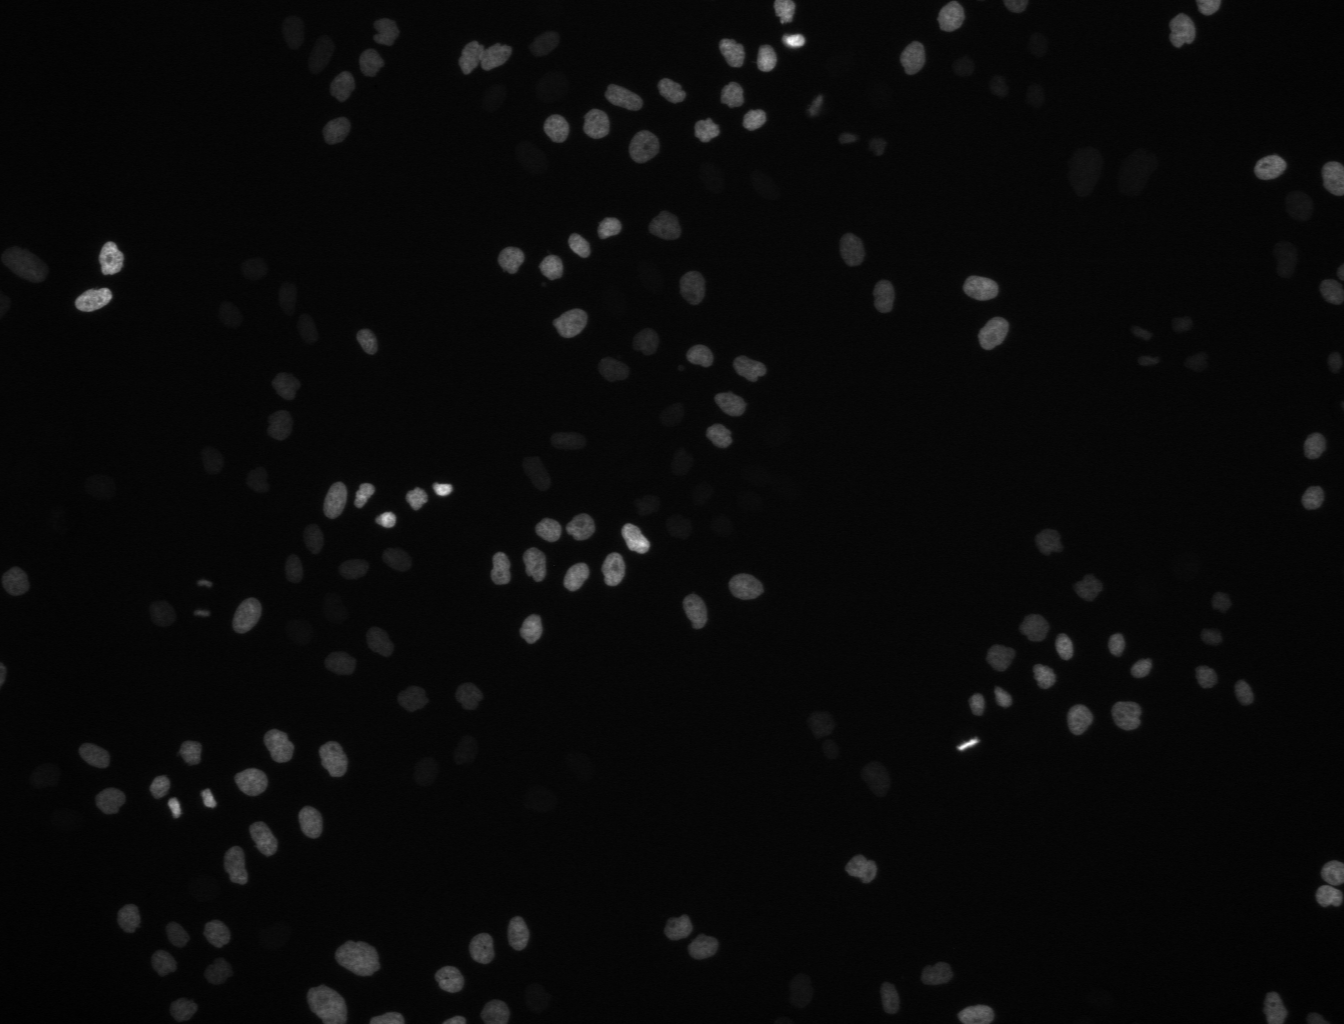
\includegraphics[width=\textwidth]{images/gmm/data/C/10.png}
        \caption{$t=10$}
        \label{fig:gmm-data-c-early}
    \end{subfigure}
    \hfill
    \begin{subfigure}{0.32\textwidth}
        \centering
        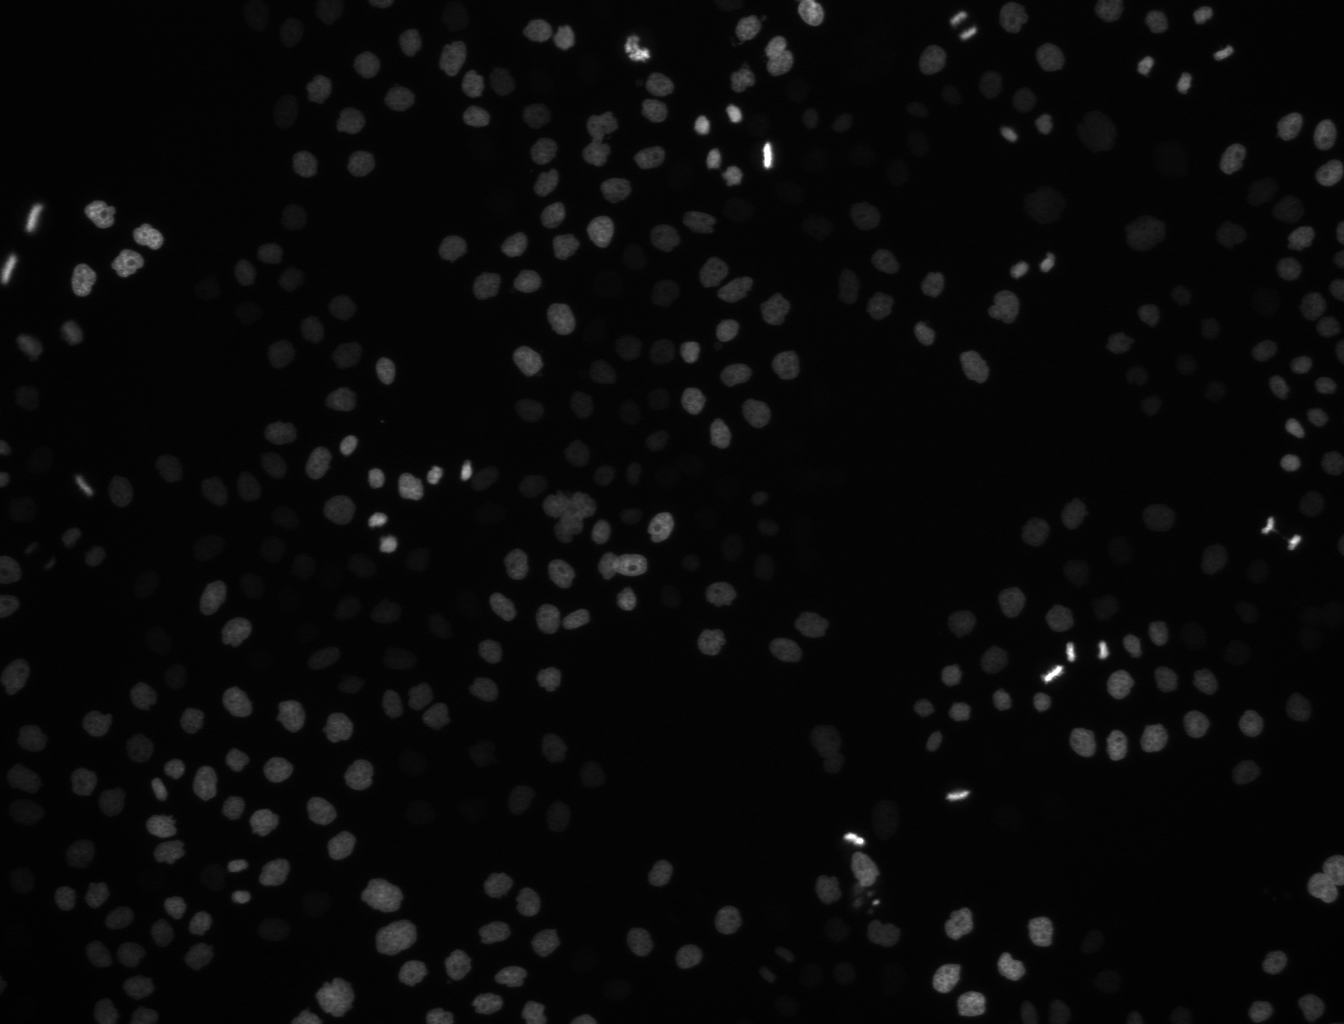
\includegraphics[width=\textwidth]{images/gmm/data/C/50.png}
        \caption{$t=50$}
        \label{fig:gmm-data-c-mid}
    \end{subfigure}
    \hfill
    \begin{subfigure}{0.32\textwidth}
        \centering
        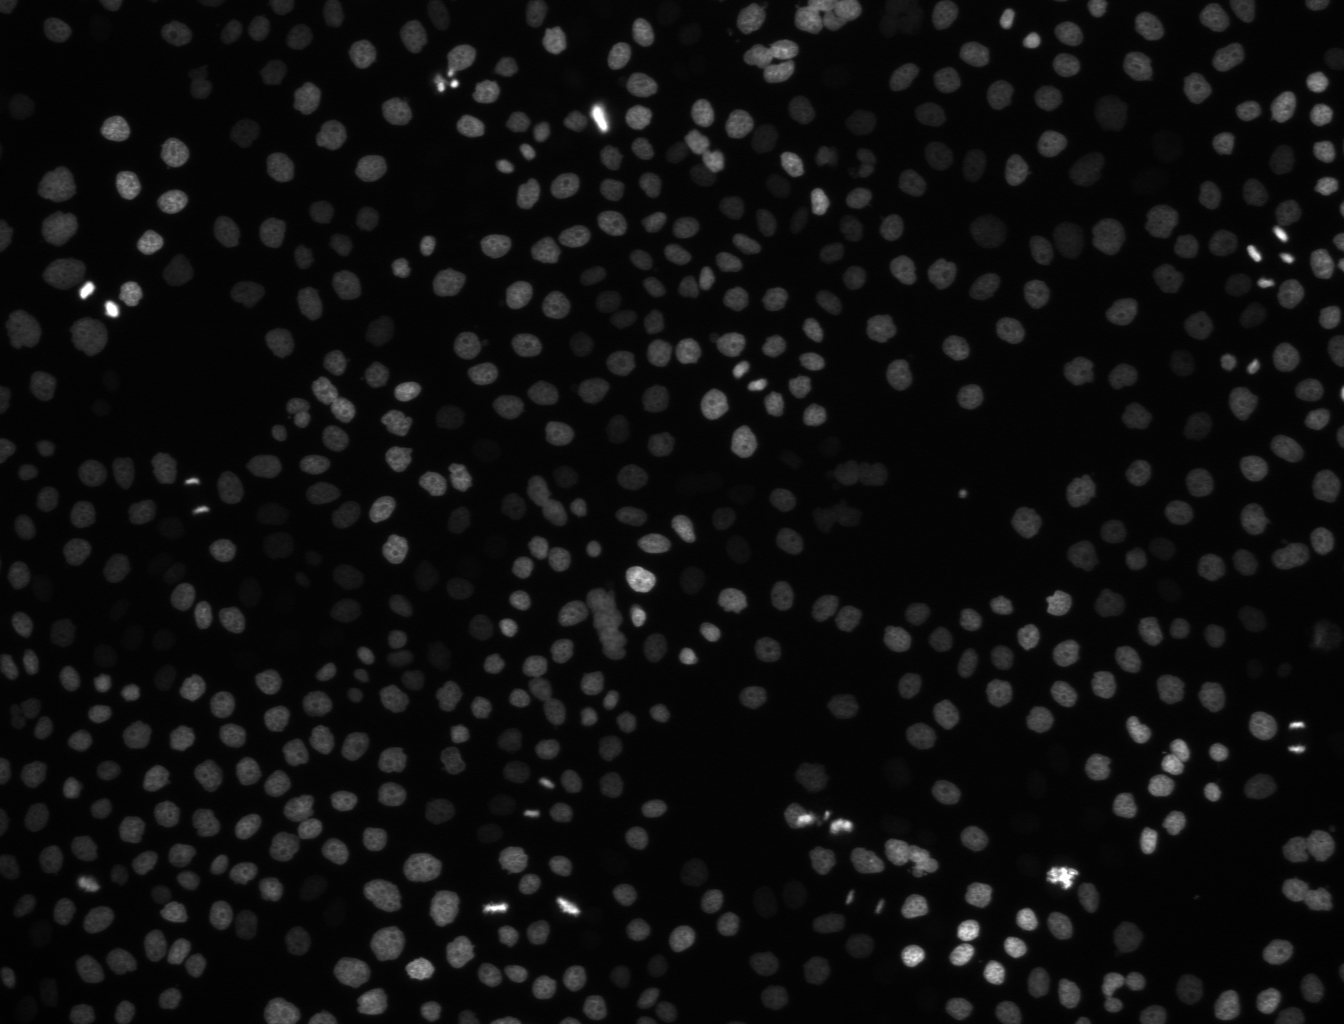
\includegraphics[width=\textwidth]{images/gmm/data/C/85.png}
        \caption{$t=85$}
        \label{fig:gmm-data-c-late}
    \end{subfigure}
    \hfill
    \caption[An excerpt of data set C]{Three slices of $2d+t$ data set C (MitoCheck). The time series shows an increase
        in cells as well as in merged/occluded objects.}
    \label{fig:gmm-data-c-three-slices}
\end{figure}

Only recently, new developments in light sheet microscopy, namely low
phototoxicity~\citep{jemielita_12_comparing} and fast, fully isotropic, high resolution
imaging~\citep{santi_11_light,weber_11_light,keller_12_light} resulted in high-quality recordings of
other organisms, such as \emph{Arabidopsis thaliana}~\citep{maizel_11_high},
zebrafish~\citep{keller_08_reconstruction} or
\emph{Drosophila}~\citep{keller_10_fast,krzic_12_multiview}, which are fit to automated processing.


\begin{figure}
    \centering
    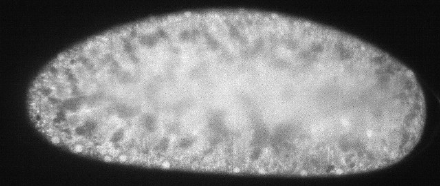
\includegraphics[width=\textwidth]{images/gmm/data/A/dataA.png}
    \caption[Two-dimensional slice of the first volume of data set A]{Two-dimensional slice of the
        first volume of $3d+t$ data set A (Drosophila, taken from \citet[43]{kausler_13_tracking}). The
        border area of the embryo contains the cell nuclei. The cytoplasm also contributes to the
        intensity. A more detailed description can be found in \cref{subsec:gmm-data}.}
    \label{fig:gmm-data-a}
\end{figure}

% Embryogenesis is the process of embryonic development and is paramount to developmental biologists' research.
% %"subject?"
% %You could say that or "paramount" "of pinnacle importance" "instrumental"

% %Developmental biologists are
% %especially interested in this phase of development, but,
% However, as yet, they lack a large scale analysis of the embryogenesis. Now, with an increasing
% amount of data available, the digitization of embryogenesis, which is a basic prerequisite for the
% quantitative analysis, becomes tangible. In addition to the impact on fundamental science, a
% quantitative analysis of the embryo could affect other research fields, \eg
% pharmacy~\citep{kunz_04_use} or medicine~\citep{kari_07_zebrafish,chakraborty_09_zebrafish}.

% While this increasing amount of data in developmental biology boosts the potential for statistical
% analysis in the field, at the same time it gives rise to the need for automated processing of data,
% as manual processing becomes infeasible~\citep{meijering_09_tracking}. In particular, developmental
% biologists are interested in the tracking~\citep{miura_05_tracking} or lineage tree generation for every cell in
% embryogenesis. While the complete embryonic lineage of the nematode \emph{Caenorhabditis elegans}
% has been reconstructed~\citep{sulston_83_embryonic}, for other organisms, such as \emph{Drosophila}
% or zebrafish, the challenge remains open. With recent advances in light sheet microscopy, namely low
% phototoxicity~\citep{jemielita_12_comparing}, fast, fully isotropic, high resolution
% imaging~\citep{santi_11_light,weber_11_light,keller_12_light}, sequences of embryonic development
% for model organisms, such as \emph{Arabidopsis thaliana}~\citep{maizel_11_high},
% zebrafish~\citep{keller_08_reconstruction} or
% \emph{Drosophila}~\citep{keller_10_fast,krzic_12_multiview}, have been acquired.

With the data available, developmental biologists are in need of reliable, automated cell-tracking
algorithms. The complete digital reconstruction of the embryo requires both high recall and high
precision. This means that no actual cell in the data should be lost in the reconstruction and every
reconstructed cell should represent an actual cell i nthe data. To this end,
\citet{kausler_12_discrete} introduced a graphical model formulation of tracking-by-assignment that
is capable of distinguishing false positive detections (oversegmentation) from true cells in regions
with low signal-to-noise ratio, but fails in case of undersegmentation, \ie multiple cells appear as
one single object in the segmentation. The handling of the latter kind of segmentation errors is the
topic of our thesis. In particular, our contributions are:
\begin{enumerate}
      \item \citet{schiegg_13_conservation} introduced a tracking-by-assignment approach,
    conservation tracking, which is able to detect merged objects based on global tracking
    information. Our contribution is the \emph{reconstruction of cell identities} in a conservation
    tracking post-processing procedure~(\cref{cha:GMM}), thus allowing for tracking in the presence
    of undersegmentation, \ie merged objects. To this end, we fit Gaussian Mixture Models to merged objects and extract
    relevant information for a tracking on the subset of merged objects.
    % \emph{cell identity} recontsrutction postprocessing procedure~(\cref{cha:GMM}) for the
    % conservation tracking method~\citep{schiegg_13_conservation}, which allows the generation of
    % valid cell tracks in the presence of merged objects
    % .
      \item We introduce a new tracking model for \emph{joint segmentation and tracking} that goes
    beyond existing tracking-by-assignment methods and states multiple, possibly conflicting
    segmentation hypotheses. Global temporal context of the tracking then determines the most
    plausible segmentation~(\cref{cha:joint}). In the fashion of
    \citet{kausler_12_discrete,schiegg_13_conservation}, we formulate our method in terms of a
    \emph{probabilistic graphical model}, which models cell-tracking constraints as well as
    segmentation consistency, and solve for global optimality.% Briefly, our method comprises of
    % \begin{enumerate}
    %     \item 
    % \end{enumerate}
\end{enumerate}

\begin{figure}
    \centering
    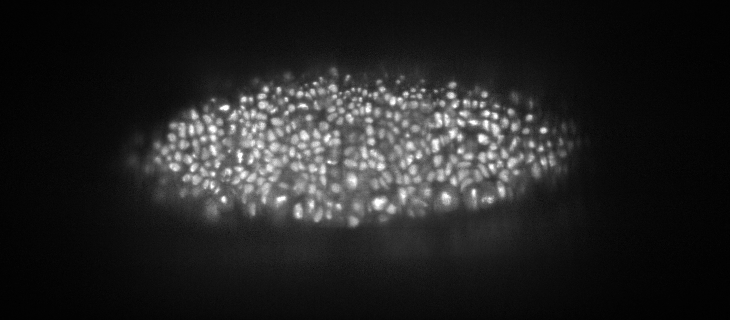
\includegraphics[width=\textwidth]{images/gmm/data/B/300-399_z30_raw_0097_0014.png}
    \caption[Two-dimensional slice of data set B]{Two-dimensional slice of data set B (Drosophila)
        at $z=15$ and $t=98$ showing the dense cell population in this $3d+t$ data set, \cf
        \cref{subsec:gmm-data} for more details.}
    \label{fig:gmm-data-b-dense-population}
\end{figure}

After a presentation of related work in the following \cref{sec:related}, we will continue with a
short introduction to probability theory and graphical models in \cref{cha:probabilistic_graphical_models}. Before we
continue with the presentation our own work in \cref{cha:GMM,cha:joint}, two existing
tracking-by-assignment methods are presented in \cref{cha:gm-in-tracking}. Finally,
\cref{cha:conclusion} summarizes our results.



\section{Related Work}
\label{sec:related}
Target tracking in general has its application in many areas, each imposing its unique requirements
on the respective tracking approach~\citep{yilmaz_06_object}. In the case of cell tracking, the
objects are both divisible and indistinguishable, and their number at each time step is not
known. This sets cell tracking apart from tracking similar, impartible
objects~\citep{smal_08_multiple}.

With a high temporal resolution, \ie the displacement of objects in consecutive time frames is small,
tracking can be interpreted as a spatio-temporal segmentation
\citep{melani_07_cells,padfield_09_spatio,dzyubachyk_10_advanced}. In general, however, the temporal
resolution cannot be assumed to be high enough and therefore most tracking algorithms follow a
two-step procedure by separating the detection/segmentation from the tracking/assignment. Within
this category, two main approaches are established.

Firstly, \emph{state space models} model observations as the result of a hidden state of the
underlying system. Most of the state space models are modified variations of the Kalman
filter~\citep{kalman_61_new,yang_06_nuclei}, notably
\citet{xiong_06_dynamical,arulampalam_02_tutorial,doucet_09_tutorial,ong_10_tracking,fox_06_nonparametric}. The
strength of state space models lies in the robustness against noise and the ability to implement
target properties, \eg velocity or size. However, their abilities are limited when it comes to
modeling an unknown number of divisible objects.

This leads us to the second approach, \emph{tracking-by-assignment}, which regards every detection
as a potential tracking target, thus allowing for the model-ling of an unknown number of divisible
objects. The difficulty is then to restrict the flexible model in order to fit the requirements of
cell tracking, \ie each cell must belong to a unique lineage and a division into more than two
children cells is impossible. Previous methods have approached this by building a hierarchical,
tracklet based tracking~\citep{bise_11_reliable,brendel_11_multiobject,li_09_learning} or by
reducing the tracking to pairs of adjacent time
frames~\citep{chen_06_automated,kachouie_07_extended,kanade_11_cell,padfield_11_coupled,lou_11_digital}. More
recently, \citet{kausler_12_discrete} introduced a graphical model formulation for
tracking-by-assignment that first builds assignment hypotheses for pairs of detections and finds a
globally optimal tracking solution with false positive detection
handling. \citet{schiegg_13_conservation} extend this approach by allowing multiple states of
detections, thus modeling merged cells.

Our proposed joint segmentation and tracking model implements multiple, competing segmentation
hypotheses and blurs the strict distinction between detection and tracking in previous
tracking-by-assignment approaches. While the concept of competing segmentation hypotheses and joint
optimization for segmentation and tracking is a novelty in cell tracking, similar approaches have
been applied in $2d$-, $3d$- and video segmentation as well as the tracking of non-divisible objects.

\citet{brendel_10_segmentation} generate a set of multiple, conflicting $2d$ segmentation hypotheses
and model them in a conflict graph, \ie edges model conflicting regions. The optimal segmentation is
determined by finding the maximum weight independent set (MWIS) in the conflict graph. Following the
same idea, \citet{ion_11_image} build the complement graph of a conflict graph, named consistency
graph. Therefore, the segmentation solution is the maximum weighted clique in the consistency
graph. In video segmentation, \citet{vazquez_10_multiple} create hypotheses for groupings of
super pixels over multiple frames with the possibility of incompatible, \ie overlapping,
hypotheses. Hypotheses are scored by their photo-metric consistencies and the best competing
segmentation is determined by a maximum a posteriori estimate on a higher-order conditional random
field.

In the context of human tracking, \citet{brendel_11_multiobject} generate competing assignment
hypotheses between target detections in adjacent time frames. The tracking solution is the MWIS on
the corresponding conflict class. \citet{hofmann_13_hypergraphs} formulate multi-object tracking
with multiple overlapping views as a generalization of the network flow. The tracking of divisible
objects, however, cannot be formulated as network flow.

Most notably and closest to our approach, \citet{funke_12_efficient} propose an algorithm for
segmenting an anisotropic $3d$ volume of branching neurons by generating segmentation hypotheses in
$2d$ slices separately and posing constraints between overlapping segmentation hypotheses. In
contrast to our model, they do not model background for their specific use-case and hence, the model
cannot be applied directly to our application where it is important to infer both whether a segment
should be activated as foreground and to which segments in the consecutive time steps it should be
linked.

Lastly, \citet{liu_13_joint} introduce a method for simultaneous cell segmentation and
classification. Starting from an oversegmentation, cell hypotheses are produced by hierarchical
merging with conflicting regions subsumed in conflict sets. Then, labeling and the final
segmentation are inferred simultaneously, subject to consistency constraints imposed by the conflict
sets. Here, contextual information is not the temporal tracking, but the label-ling of the cells.


% propose a $3d$ segmentation of
% neurons based on multiple, possibly conflicting $2d$ segmentation hypotheses (superpixels) at every
% slice of the $3d$ stack. Assignments hypotheses between superpixels of adjacent slices for
% continuation, branching and endings of neurons are scored and the resulting $3d$ segmentation is the
% best scoring overall solution that fulfills consistency constraints for both segmentation and
% assignments.



%%% Local Variables: 
%%% mode: latex
%%% TeX-master: "../main"
%%% End: 

